\chapter{予備実験}
\label{chap:pre_experiment}

この章では本研究で行った予備実験について述べる.
本予備実験の目的は, 本実験の際に本システムの処理が妥当であることを証明するためのものとした.
まず笑顔データを作成する際のフレーム数および秒数の指定についてシステムの予備実験を行い,
次に笑顔の動画データを収集する際に使用する採用モデルの評価を行なった.
\section{表情を作るのかかる時間}
本システムはユーザーの顔を認識し, その表情の変化を記録し表情分析を行う.
ユーザーへ笑顔動画データをフィードバックをする際には, 人間が表情の変化を認識することができるフレーム数を
確保しなければならない.
織田らの瞬間的に変化する表情を人がどの程度正確に認知をすることができるのかを検証した研究では,
笑顔と怒りの場合は, 200m\/s まで高い認知をすることが可能であると述べている.\cite{織田朝美2005表情の瞬間的変化の認知}

\subsection{実験}
本システムを起動し, 自身のラップトップPCがどれだけのフレームレート(fps)でユーザーの記録を行うことができるのかを検証する.
取得したfpsの値を用いて, 織田らが明示した1フレーム辺りの表示時間が200ms  以上,
つまりミリフレームレート(fpms)が200以下であることを確認する.

\subsection{結果}
\begin{itemize}
\item 実行結果
\setlength{\parskip}{20pt}
\begin{lstlisting}
start_from_webcam
FPSの設定値、video.get(cv2.CAP_PROP_FPS) : 20.0
\end{lstlisting}
%複数の時は以下のように
%\item 実行コマンド
%\begin{lstlisting}
%$ python dsfsa.py mode_num
%\end{lstlisting}
\end{itemize}
本システムにおけるfpsは20であったため, 1秒間に20フレームを取得することができている.
よって,これをミリフレームレート(fpms)に変換すると,
\begin{equation}
\label{fpms}
 fpms = \frac{1000.0}{20.0} = 50.0
\end{equation}
となる.
よって, 人が認知に必要な200ms以上フレームを取得し, 表示することができているためこのシステムは
人の表情の変化を知覚する条件を満たしていることが証明できた.


\section{OpenCVを使った笑顔検出の妥当性}
本システムでは収集した笑顔動画データを解析する際には, Cambridge大学が開発したオープンソースの
OpenFace を使用している. 顔パーツの位置や, Facial Action Units (以下FAU)によって表情を
判断するパーツの動きの強度を取得することが可能である.
しかし, 開発途中のオープンソースおよび有用なデータを1フレームに対して, 711個データを取得するため
処理時間が長くなってしまう.

pythonの中に含まれる, cProfileを使用して静止画,
1フレームの時間を取得すると, 平均約4secの処理時間がかかることが判明し, さらに本研究で採用している20フレーム分の処理を行なった場合,
20秒の処理時間を要することが判明した.
以上のことより, 笑顔動画データを作成するためのフレーム取得にはより処理速度の速いOpenCVの中に含まれる
haarcascades\/ haarcascade\_ smile.xmlの笑顔判定モデルを使用した.

 \begin{itemize}
   \setlength{\parskip}{20pt}      %4. 段落間余白
 \item 処理時間時間計測
 \begin{lstlisting}
 $ python -m cProfile -s tottime dsfsa.py
 \end{lstlisting}
 \end{itemize}

\subsection{実験}
OpenCvの笑顔判定モデルを使用して, 人が映っている動画データに対して笑顔検出を行う.
笑顔のフレームを一番最後に5フレーム含み, 全体20秒の笑顔動画データを作成する.
作成した笑顔動画データに対してOpenFaceの処理を行い, 最後のフレームに対して笑顔のFAUである
FAU06(眼窩部眼輪筋)とFAU12(大頬骨筋)の判定値が検出できるかどうかを判定する.
実験はテストデータ3つに対して行った.

\subsection{結果}
OpenCVの笑顔認識モデルを使用して作成した笑顔動画データに対して, OpenFaceの処理を行なった結果を
図\ref{fig:preex1},\ref{fig:preex2},\ref{fig:preex3} に出力した.
各データともに, FAU06およびFAU12(大頬骨筋)の値を検出することができた.
よってデータ収集の際に, OpenCVの笑顔判別器を使用してデータ収集をすることは可能であることがわかった.

\begin{figure}[htbp]
  \setlength\intextsep{0pt}
    \begin{center}
       \fbox{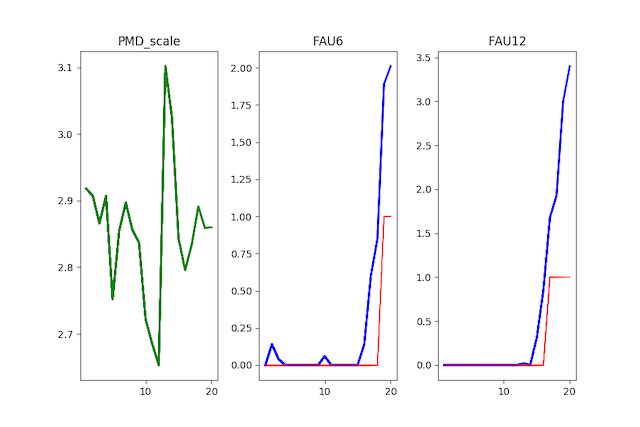
\includegraphics[width=150mm,bb=0 0 600 427]{preex1.jpg}}
    \end{center}
    \caption{笑顔動画データ1}
    \label{fig:preex1}
\end{figure}

\begin{figure}[htbp]
  \setlength\intextsep{0pt}
    \begin{center}
       \fbox{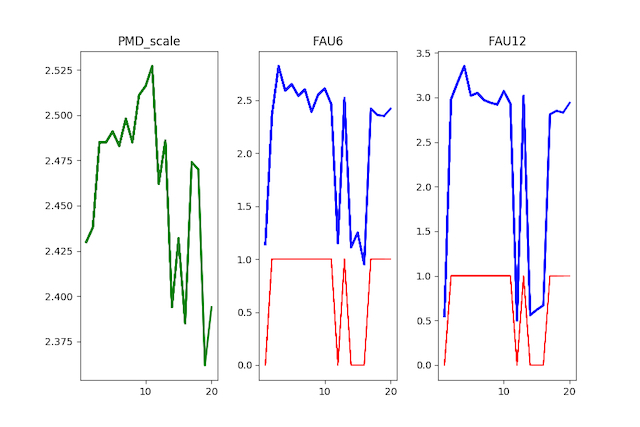
\includegraphics[width=150mm,bb=0 0 640 427]{preex2.jpg}}
    \end{center}
    \caption{笑顔動画データ2}
    \label{fig:preex2}
\end{figure}
\begin{figure}[htbp]
  \setlength\intextsep{0pt}
    \begin{center}
       \fbox{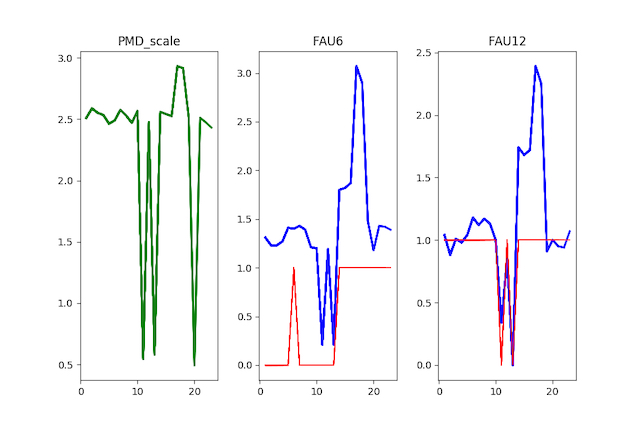
\includegraphics[width=150mm,bb=0 0 640 427]{preex3.jpg}}
    \end{center}
    \caption{笑顔動画データ3}
    \label{fig:preex3}
\end{figure}

\section{実験の結果・まとめ}
本章では, 本システムが実験をする際の条件を満たしているかの予備実験を行なった.
次章では本システムを用いた評価実験について述べる.
